\documentclass[tikz, preview]{standalone}

\usepackage{amsfonts, amsthm, amssymb, amsmath, stmaryrd, etoolbox}
\usepackage{tikz}
\usepackage[all,2cell]{xy}
\usetikzlibrary{matrix,arrows,shapes,decorations.markings,decorations.pathreplacing}
\definecolor{rewritecolor}{rgb}{0,.9,1}
\tikzset{rewritenode/.style={shape=circle,fill=rewritecolor,scale=0.25,font=\Huge}}
\tikzset{RWopen/.style={shape=circle,draw=black,fill=white,scale=0.5,font=\Huge}}
\tikzset{RWclosed/.style={shape=circle,fill=black,scale=0.5,font=\Huge}}
\tikzset{CDnode/.style={shape=circle,fill=white,scale=.5}}
\tikzset{zxgreen/.style={shape=circle,draw,thick,fill=green}}
\tikzset{zxred/.style={shape=circle,draw,thick,fill=red}}
\tikzset{zxyellow/.style={shape=rectangle,draw,thick,fill=yellow}}
\tikzset{zxdiamond/.style={shape=diamond,fill=black,inner sep=2.75}}
\tikzset{zxopen/.style={shape=circle,draw,thick,inner sep=2pt}}
\tikzset{->-/.style={decoration={markings,mark=at position .5 with {\arrow{>}}},postaction={decorate}}}
\tikzset{->-pos/.style={decoration={
			markings,
			mark=at position #1 with {\arrow{>}}},postaction={decorate}}}


\begin{document}
\[
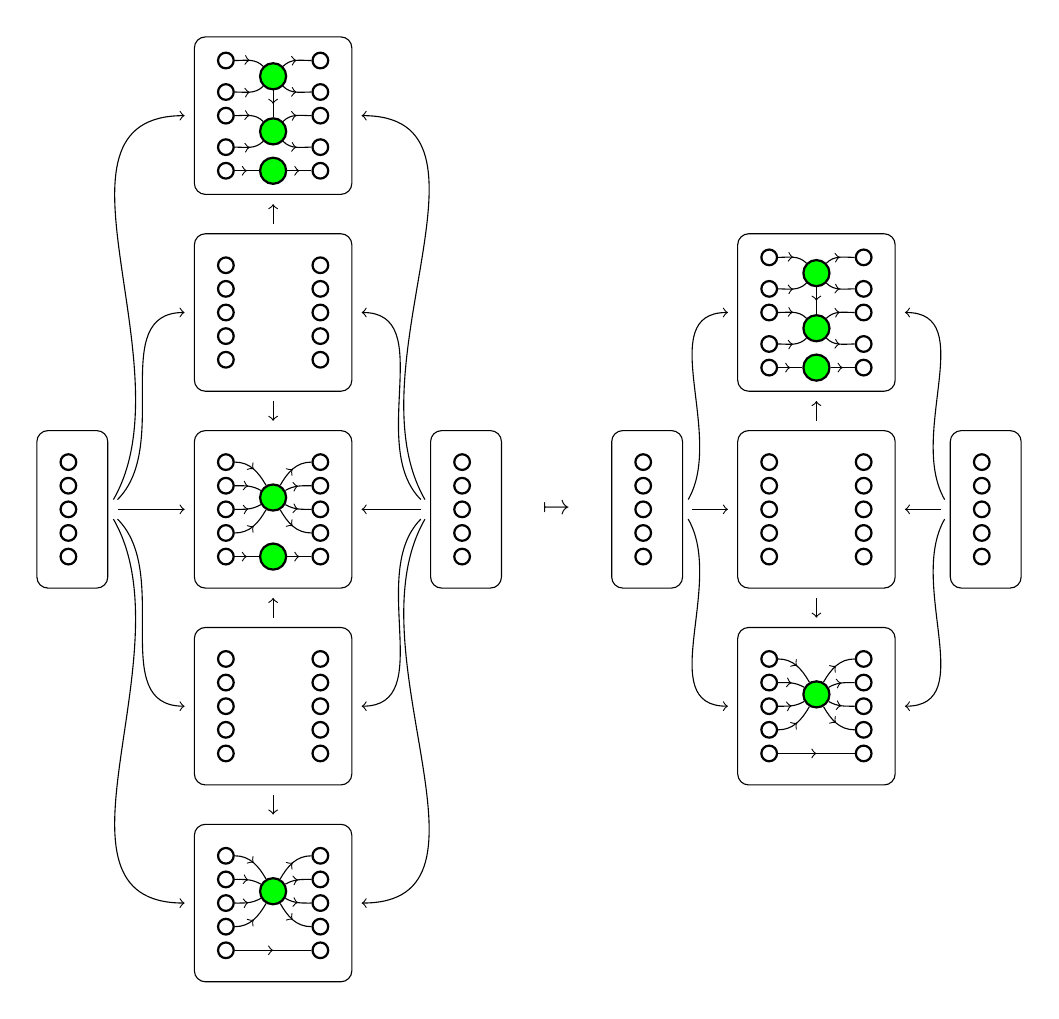
\begin{tikzpicture}
%
%
% BEGIN LEFT HAND SIDE
% BEGIN LEFT HAND SIDE
% BEGIN LEFT HAND SIDE
% BEGIN LEFT HAND SIDE
% BEGIN LEFT HAND SIDE
%
%
\begin{scope}[shift={(-2,0.1)}]
%
% 
% UP UP SCOPE -- LHS
% 
%
\begin{scope}[shift={(0,-0.4)}]
\node [zxgreen] (v1) at (0,0) {};
\node [zxopen] (v2) at (-0.6,0.2) {};
\node [zxopen] (v3) at (-0.6,-0.2) {};
\node [zxopen] (v4) at (0.6,0.2) {};
\node [zxopen] (v5) at (0.6,-0.2) {};
\draw [->-] (v2) to [out=0,in=135] (v1);
\draw [->-]  (v3) to [out=0,in=-135] (v1);
\draw [->-]  (v1) to [out=45,in=180] (v4);
\draw [->-]  (v1) to [out=-45,in=180] (v5);
%
\node [zxgreen] (v6) at (0,-0.7) {};
\node [zxopen] (v7) at (-0.6,-0.5) {};
\node [zxopen] (v8) at (-0.6,-0.9) {};
\node [zxopen] (v9) at (0.6,-0.5) {};
\node [zxopen] (v10) at (0.6,-0.9) {};
\draw [->-]  (v7) to [out=0,in=135] (v6);
\draw [->-]  (v8) to [out=0,in=-135] (v6);
\draw [->-]  (v6) to [out=45,in=180] (v9);
\draw [->-] (v6) to [out=-45,in=180] (v10);
\draw [->-]  (v1) to (v6);
%
\node [zxopen] (v11) at (-0.6,-1.2) {};
\node [zxgreen] (v12) at (0,-1.2) {};
\node [zxopen] (v13) at (0.6,-1.2) {};
\draw [->-] (v11) to (v12);
\draw [->-] (v12) to (v13);
%
\node (r1) at (-1,0.5) {};
\node (r2) at (1,-1.5) {};
\draw [rounded corners] (r1) rectangle (r2);
%
\node (a1) at (0,-1.5) {};
\node (a_up_up_left) at (-1,-0.5) {};
\node (a_up_up_right) at (1,-0.5) {};
\end{scope}
%
%
% UP SCOPE  -- LHS
%
%
\begin{scope}[shift={(0,-2.9)}]
\node [zxopen] (v2) at (-0.6,0.1) {};
\node [zxopen] (v3) at (-0.6,-0.2) {};
\node [zxopen] (v4) at (0.6,0.1) {};
\node [zxopen] (v5) at (0.6,-0.2) {};
%
\node [zxopen] (v7) at (-0.6,-0.5) {};
\node [zxopen] (v8) at (-0.6,-0.8) {};
\node [zxopen] (v9) at (0.6,-0.5) {};
\node [zxopen] (v10) at (0.6,-0.8) {};
%
\node [zxopen] (v11) at (-0.6,-1.1) {};
\node [zxopen] (v13) at (0.6,-1.1) {};
%
\node (r1) at (-1,0.5) {};
\node (r2) at (1,-1.5) {};
\draw [rounded corners] (r1) rectangle (r2);
%
\node (a2) at (0,0.5) {};
\node (a3) at (0,-1.5) {};
\node (a_up_left) at (-1,-0.5) {};
\node (a_up_right) at (1,-0.5) {};
\end{scope}
%
%
% MID SCOPE -- LHS
%
%
\begin{scope}[shift={(0,-5.4)}]
\node [zxgreen] (v1) at (0,-0.35) {};
\node [zxopen] (v2) at (-0.6,0.1) {};
\node [zxopen] (v3) at (-0.6,-0.2) {};
\node [zxopen] (v4) at (0.6,0.1) {};
\node [zxopen] (v5) at (0.6,-0.2) {};
\draw [->-] (v2) to [out=0,in=120] (v1);
\draw [->-]  (v3) to [out=0,in=150] (v1);
\draw [->-]  (v1) to [out=60,in=180] (v4);
\draw [->-]  (v1) to [out=30,in=180] (v5);
%
\node [zxopen] (v7) at (-0.6,-0.5) {};
\node [zxopen] (v8) at (-0.6,-0.8) {};
\node [zxopen] (v9) at (0.6,-0.5) {};
\node [zxopen] (v10) at (0.6,-0.8) {};
\draw [->-]  (v7) to [out=0,in=-150] (v1);
\draw [->-]  (v8) to [out=0,in=-120] (v1);
\draw [->-]  (v1) to [out=-30,in=180] (v9);
\draw [->-] (v1) to [out=-60,in=180] (v10);
%
\node [zxopen] (v11) at (-0.6,-1.1) {};
\node [zxgreen] (v12) at (0,-1.1) {};
\node [zxopen] (v13) at (0.6,-1.1) {};
\draw [->-] (v11) to (v12);
\draw [->-] (v12) to (v13);
%
\node (r1) at (-1,0.5) {};
\node (r2) at (1,-1.5) {};
\draw [rounded corners] (r1) rectangle (r2);
%
\node (a4) at (0,0.5) {};
\node (a5) at (0,-1.5) {};
\node (a_mid_left) at (-1,-0.5) {};
\node (a_mid_right) at (1,-0.5) {};
\end{scope}
%
%
% DOWN SCOPE -- LHS
%
%
\begin{scope}[shift={(0,-7.9)}]
\node [zxopen] (v2) at (-0.6,0.1) {};
\node [zxopen] (v3) at (-0.6,-0.2) {};
\node [zxopen] (v4) at (0.6,0.1) {};
\node [zxopen] (v5) at (0.6,-0.2) {};
%
\node [zxopen] (v7) at (-0.6,-0.5) {};
\node [zxopen] (v8) at (-0.6,-0.8) {};
\node [zxopen] (v9) at (0.6,-0.5) {};
\node [zxopen] (v10) at (0.6,-0.8) {};
%
\node [zxopen] (v11) at (-0.6,-1.1) {};
\node [zxopen] (v13) at (0.6,-1.1) {};
%
\node (r1) at (-1,0.5) {};
\node (r2) at (1,-1.5) {};
\draw [rounded corners] (r1) rectangle (r2);
%
\node (a6) at (0,0.5) {};
\node (a7) at (0,-1.5) {};
\node (a_down_left) at (-1,-0.5) {};
\node (a_down_right) at (1,-0.5) {};
\end{scope}
%
%
% DOWN DOWN SCOPE -- LHS
%
%
\begin{scope}[shift={(0,-10.4)}]
\node [zxgreen] (v1) at (0,-0.35) {};
\node [zxopen] (v2) at (-0.6,0.1) {};
\node [zxopen] (v3) at (-0.6,-0.2) {};
\node [zxopen] (v4) at (0.6,0.1) {};
\node [zxopen] (v5) at (0.6,-0.2) {};
\draw [->-] (v2) to [out=0,in=120] (v1);
\draw [->-]  (v3) to [out=0,in=150] (v1);
\draw [->-]  (v1) to [out=60,in=180] (v4);
\draw [->-]  (v1) to [out=30,in=180] (v5);
%
\node [zxopen] (v7) at (-0.6,-0.5) {};
\node [zxopen] (v8) at (-0.6,-0.8) {};
\node [zxopen] (v9) at (0.6,-0.5) {};
\node [zxopen] (v10) at (0.6,-0.8) {};
\draw [->-]  (v7) to [out=0,in=-150] (v1);
\draw [->-]  (v8) to [out=0,in=-120] (v1);
\draw [->-]  (v1) to [out=-30,in=180] (v9);
\draw [->-] (v1) to [out=-60,in=180] (v10);
%
\node [zxopen] (v11) at (-0.6,-1.1) {};
\node [zxopen] (v13) at (0.6,-1.1) {};
\draw [->-] (v11) to (v13);
%
\node (r1) at (-1,0.5) {};
\node (r2) at (1,-1.5) {};
\draw [rounded corners] (r1) rectangle (r2);
%
\node (a8) at (0,0.5) {};
\node (a_down_down_left) at (-1,-0.5) {};
\node (a_down_down_right) at (1,-0.5) {};
\end{scope}
%
%
% INPUTS -- LHS
%
%
\begin{scope}[shift={(-3.1,-5.4)}]
\node [zxopen] at (0.5,0.1) {};
\node [zxopen] at (0.5,-0.2) {};
\node [zxopen] at (0.5,-0.5) {};
\node [zxopen] at (0.5,-0.8) {};
\node [zxopen] at (0.5,-1.1) {};
%
\node (r1) at (0.1,0.5) {};
\node (r2) at (1,-1.5) {};
\draw [rounded corners] (r1) rectangle (r2);
%
\node (a_inputs) at (1,-0.5) {};
\end{scope}
%
%
% OUTPUTS -- LHS
%
%
\begin{scope}[shift={(1.9,-5.4)}]
\node [zxopen] at (0.5,0.1) {};
\node [zxopen] at (0.5,-0.2) {};
\node [zxopen] at (0.5,-0.5) {};
\node [zxopen] at (0.5,-0.8) {};
\node [zxopen] at (0.5,-1.1) {};
%
\node (r1) at (0.1,0.5) {};
\node (r2) at (1,-1.5) {};
\draw [rounded corners] (r1) rectangle (r2);
%
\node (a_outputs) at (0.1,-0.5) {};
\end{scope}
%
%
% (CO)SPAN ARROWS
%
%
\draw [->]  (a2) edge (a1);
\draw [->] (a3) edge (a4);
\draw [->] (a6) edge (a5);
\draw [->] (a7) edge (a8);
\draw [->] (a_inputs) to [out=60,in=180] (a_up_up_left);
\draw [->] (a_inputs) to [out=45,in=180] (a_up_left);
\draw [->] (a_inputs) to [out=0,in=180] (a_mid_left);
\draw [->] (a_inputs) to [out=-45,in=180] (a_down_left);
\draw [->] (a_inputs) to [out=-60,in=180] (a_down_down_left);
\draw [->] (a_outputs) to [out=120,in=0] (a_up_up_right);
\draw [->] (a_outputs) to [out=135,in=0] (a_up_right);
\draw [->] (a_outputs) to [out=180,in=0] (a_mid_right);
\draw [->] (a_outputs) to [out=-135,in=0] (a_down_right);
\draw [->] (a_outputs) to [out=-120,in=0] (a_down_down_right);
%
%
% END LEFT HAND SIDE
% END LEFT HAND SIDE
% END LEFT HAND SIDE
% END LEFT HAND SIDE
% END LEFT HAND SIDE
%
\end{scope}
%
%
%   BEGIN RIGHT HAND SIDE
%   BEGIN RIGHT HAND SIDE
%   BEGIN RIGHT HAND SIDE
%   BEGIN RIGHT HAND SIDE
%   BEGIN RIGHT HAND SIDE
%
%
\begin{scope}[shift={(4.9,-2.6)}]
%
%
% UP SCOPE --RHS
%
%
\begin{scope}[shift={(0,-0.2)}]
\node [zxgreen] (v1) at (0,0) {};
\node [zxopen] (v2) at (-0.6,0.2) {};
\node [zxopen] (v3) at (-0.6,-0.2) {};
\node [zxopen] (v4) at (0.6,0.2) {};
\node [zxopen] (v5) at (0.6,-0.2) {};
\draw [->-] (v2) to [out=0,in=135] (v1);
\draw [->-]  (v3) to [out=0,in=-135] (v1);
\draw [->-]  (v1) to [out=45,in=180] (v4);
\draw [->-]  (v1) to [out=-45,in=180] (v5);
%
\node [zxgreen] (v6) at (0,-0.7) {};
\node [zxopen] (v7) at (-0.6,-0.5) {};
\node [zxopen] (v8) at (-0.6,-0.9) {};
\node [zxopen] (v9) at (0.6,-0.5) {};
\node [zxopen] (v10) at (0.6,-0.9) {};
\draw [->-]  (v7) to [out=0,in=135] (v6);
\draw [->-]  (v8) to [out=0,in=-135] (v6);
\draw [->-]  (v6) to [out=45,in=180] (v9);
\draw [->-] (v6) to [out=-45,in=180] (v10);
\draw [->-]  (v1) to (v6);
%
\node [zxopen] (v11) at (-0.6,-1.2) {};
\node [zxgreen] (v12) at (0,-1.2) {};
\node [zxopen] (v13) at (0.6,-1.2) {};
\draw [->-] (v11) to (v12);
\draw [->-] (v12) to (v13);
%
%
\node (r1) at (-1,0.5) {};
\node (r2) at (1,-1.5) {};
\draw [rounded corners] (r1) rectangle (r2);
%
\node (a1) at (0,-1.5) {};
\node (a_up_left) at (-1,-0.5) {};
\node (a_up_right) at (1,-0.5) {};
\end{scope}
%
%
% MID SCOPE -- RHS
%
%
\begin{scope}[shift={(0,-2.7)}]
\node [zxopen] (v2) at (-0.6,0.1) {};
\node [zxopen] (v3) at (-0.6,-0.2) {};
\node [zxopen] (v4) at (0.6,0.1) {};
\node [zxopen] (v5) at (0.6,-0.2) {};
%
\node [zxopen] (v7) at (-0.6,-0.5) {};
\node [zxopen] (v8) at (-0.6,-0.8) {};
\node [zxopen] (v9) at (0.6,-0.5) {};
\node [zxopen] (v10) at (0.6,-0.8) {};
%
\node [zxopen] (v11) at (-0.6,-1.1) {};
\node [zxopen] (v13) at (0.6,-1.1) {};
%
\node (r1) at (-1,0.5) {};
\node (r2) at (1,-1.5) {};
\draw [rounded corners] (r1) rectangle (r2);
%
\node (a2) at (0,0.5) {};
\node (a3) at (0,-1.5) {};
\node (a_mid_left) at (-1,-0.5) {};
\node (a_mid_right) at (1,-0.5) {};
\end{scope}
%
%
% DOWN SCOPE --RHS
%
%
\begin{scope}[shift={(0,-5.2)}]
\node [zxgreen] (v1) at (0,-0.35) {};
\node [zxopen] (v2) at (-0.6,0.1) {};
\node [zxopen] (v3) at (-0.6,-0.2) {};
\node [zxopen] (v4) at (0.6,0.1) {};
\node [zxopen] (v5) at (0.6,-0.2) {};
\draw [->-] (v2) to [out=0,in=120] (v1);
\draw [->-]  (v3) to [out=0,in=150] (v1);
\draw [->-]  (v1) to [out=60,in=180] (v4);
\draw [->-]  (v1) to [out=30,in=180] (v5);
%
\node [zxopen] (v7) at (-0.6,-0.5) {};
\node [zxopen] (v8) at (-0.6,-0.8) {};
\node [zxopen] (v9) at (0.6,-0.5) {};
\node [zxopen] (v10) at (0.6,-0.8) {};
\draw [->-]  (v7) to [out=0,in=-150] (v1);
\draw [->-]  (v8) to [out=0,in=-120] (v1);
\draw [->-]  (v1) to [out=-30,in=180] (v9);
\draw [->-] (v1) to [out=-60,in=180] (v10);
%
\node [zxopen] (v11) at (-0.6,-1.1) {};
\node [zxopen] (v13) at (0.6,-1.1) {};
\draw [->-] (v11) to (v13);
%
\node (r1) at (-1,0.5) {};
\node (r2) at (1,-1.5) {};
\draw [rounded corners] (r1) rectangle (r2);
%
\node (a4) at (0,0.5) {};
\node (a_down_left) at (-1,-0.5) {};
\node (a_down_right) at (1,-0.5) {};
\end{scope}
%
%
% INPUTS -- RHS
%
%
\begin{scope}[shift={(-2.7,-2.7)}]
\node [zxopen] at (0.5,0.1) {};
\node [zxopen] at (0.5,-0.2) {};
\node [zxopen] at (0.5,-0.5) {};
\node [zxopen] at (0.5,-0.8) {};
\node [zxopen] at (0.5,-1.1) {};
%
\node (r1) at (0.1,0.5) {};
\node (r2) at (1,-1.5) {};
\draw [rounded corners] (r1) rectangle (r2);
%
\node (a_inputs) at (1,-0.5) {};
\end{scope}
%
%
% OUTPUTS -- RHS
%
%
\begin{scope}[shift={(1.6,-2.7)}]
\node [zxopen] at (0.5,0.1) {};
\node [zxopen] at (0.5,-0.2) {};
\node [zxopen] at (0.5,-0.5) {};
\node [zxopen] at (0.5,-0.8) {};
\node [zxopen] at (0.5,-1.1) {};
%
\node (r1) at (0.1,0.5) {};
\node (r2) at (1,-1.5) {};
\draw [rounded corners] (r1) rectangle (r2);
%
\node (a_outputs) at (0.1,-0.5) {};
\end{scope}
%
%
% (CO)SPAN ARROWS
%
%
\draw [->]  (a2) edge (a1);
\draw [->] (a3) edge (a4);
\draw[->] (a_inputs) to [out=60,in=180] (a_up_left);
\draw[->] (a_inputs) to [out=0,in=180] (a_mid_left);
\draw[->] (a_inputs) to [out=-60,in=180] (a_down_left);
\draw[->] (a_outputs) to [out=120,in=0] (a_up_right);
\draw[->] (a_outputs) to [out=180,in=0] (a_mid_right);
\draw[->] (a_outputs) to [out=-120,in=0] (a_down_right);
%
%
% END RIGHT HAND SIDE 
% END RIGHT HAND SIDE 
% END RIGHT HAND SIDE 
% END RIGHT HAND SIDE 
% END RIGHT HAND SIDE 
%
%
\end{scope}
%
%
% EQUALS SIGN
% EQUALS SIGN
% EQUALS SIGN
% EQUALS SIGN
% EQUALS SIGN
%
%
\node at (1.6,-5.8) {$\mapsto$};
\end{tikzpicture}
\]
\end{document}
